\begin{figure}[tbp]
\begin{center}
\includegraphics[width=0.48\textwidth]{cl_correlation_z1_z2.eps}
\end{center}
\vspace{-0.7cm}
\caption{The cross correlation r between reconstructed kSZ $P_{\hat \Theta_{kSZ}}$ 
and real kSZ $P_{\Theta_{kSZ}}$.
    (Dashed line) kSZ calculated from foreground filtered 21cm density field $\delta_{fs}$;
    (Solid line) kSZ calculated from tidal reconstructed density field.
    (Blue lines) take into account of redshift space distortions.
}
\label{fig:r}
\end{figure}
With noise substracted 21cm density field, we are able to have detectable cross correlations for $\ell\gtrsim 800$. 
However, we are also interested in large scale baryon distributions, 
which is free from the complicated activities happen in smaller scales.  
We use Cosmic Tidal Reconstruction to recover correlations for small $\ell$ 
and improve correlations for intermediate $\ell$.
%Since the loss of large scale information in z dDDddirection will reduce the cross correlation with small $\ell$ and influence the performance on large $\ell$. 
This is one of the first application of its 3D version. 
\subsection{Algorithm}
The fundamental idea of Cosmic Tidal Reconstruction is that 
the evolution of small scale structure is modulated by large scale 
gravitational force. We can select this effect and solve for the large scale potential. 


Main Procedure:\noindent

Consider only the anisotropic influence from tidal force, 
the distortions on power spectrum \cite{2015:zhu} can linearly be calculated as  
\begin{eqnarray}
\label{eq:powerdistort}
\delta P(\bm{k},\tau)|_{t_{ij}}&=&
\hat{k}^i\hat{k}^jt_{ij}^{(0)}P_{1s}(k,\tau)f(k,\tau)
\end{eqnarray}
where f is the linear coupling function;
$P_{1s}(k,\tau)$ is the theoretical small scale linear powerspectrum; 
and $\delta P(\bm{k},\tau)$ is the real distortion from observations. 

Hence we can solve for the unknown quantity $t_{ij}$, 
which is the tidal force tensor defined as 
\begin{eqnarray}
\label{eq:tij}
t_{ij}=\Phi_{L,ij}-\nabla^2\Phi_L\delta^D_{ij}/3
\end{eqnarray}
$\Phi_{L,ij}$ is the second derivative of large scale potential, 
$\delta^D$ is the Dirac function.

With $t_{ij}$, we calculate the variance of large scale potential $\Phi_L$  
and get the large scale density contrast $\kappa_\mathrm{3D}$.
\begin{eqnarray}
    \label{eq:largepoten}
\kappa_\mr{3D}\sim\nabla^2\Phi_L=\frac{3}{2}\frac{\partial_i\partial_j}{\nabla^2}t_{ij}
\end{eqnarray}

Since $f(k,\tau)$ increase with k in our interested scales, 
the distortions are more obvious in small scales. 
Therefore, the method mainly use the quadratic statistics on small scales to recover the large scale density field. 
It works best for close linear regions.


Detailed steps:\noindent

(1) Gaussianize the field, taking 
$\delta_g=\mathrm{ln}(1+\delta)$. 
This is to allieviate the problem that filter $W_i$ in Eq.(\ref{eq:wi}) heavily weights high density regions.

(2) Following gravitational lensing procedures, decompose the symmetric, traceless tidal force tensor into 5 components, 
\begin{eqnarray}
t_{ij}=\left( \begin{array}{ccc}
\gamma_{1}-\gamma_{z} & \gamma_{\times} & \gamma_{2}\\
\gamma_{\times} & -\gamma_{1}-\gamma_{z} & \gamma_{y}\\
\gamma_{2} & \gamma_{y} & 2\gamma_z
\end{array} \right).
\end{eqnarray}

(3) Select density distortions caused by tidal force, 
by convolving $\delta_g$ with a filter $W_i$ 
deduced from Eq.(\ref{eq:powerdistort}) 
\begin{eqnarray}
\delta^{w_i}_g(\bm{k})=W_i(\bm{k})\delta_g(\bm{k}) 
\end{eqnarray}

\begin{eqnarray}
\label{eq:wi}
W_i(\bm{k})=i (\frac{P(k)f(k)}{P_{tot}^2(k)})^{\frac{1}{2}}\frac{k_i}{k}
=S(k)\frac{k_i}{k}\nonumber
\end{eqnarray}
where i indicates $\hat x,\hat y,\hat z$ directions, 
$f(k)=2\alpha(\tau)-\beta(\tau)d\ln P/d\ln k$ is again the coupling function, 
with $\alpha$ and $\beta$ related to linear growth funcion \cite{2015:zhu}, 
and calculated to be (0.6, 1.3) for $z=1$ and (0.4, 0.9) for $z=2$.
$P_{tot}=P+P_{noise}$ is observed matter powerspectrum, 
P is theoretical matter powerspectrum,
%\footnote{The value of $S(k)$ on different scales could be seen in Appendix 1.}

(4) Estimate the 5 tidal tensor components from quadratic statistics.
\begin{eqnarray}
\label{eq:gamma}
\hat{\gamma}_1(\bm{x})&=&
[{\delta}^{w_1}_g(\bm{x}){\delta}^{w_1}_g(\bm{x})-
{\delta}^{w_2}_g(\bm{x}){\delta}^{w_2}_g(\bm{x})],\nonumber\\
\hat{\gamma}_2(\bm{x})&=&
[2{\delta}^{w_1}_g(\bm{x}){\delta}^{w_2}_g(\bm{x})],\nonumber\\
\hat{\gamma}_x(\bm{x})&=&
[2{\delta}^{w_1}_g(\bm{x}){\delta}^{w_3}_g(\bm{x})],\\
\hat{\gamma}_y(\bm{x})&=&
[2{\delta}^{w_2}_g(\bm{x}){\delta}^{w_3}_g(\bm{x})],\nonumber\\
\hat{\gamma}_z(\bm{x})&=&
[(2{\delta}^{w_3}_g(\bm{x}){\delta}^{w_3}_g(\bm{x})-
{\delta}^{w_1}_g(\bm{x}){\delta}^{w_1}_g(\bm{x})-
{\delta}^{w_2}_g(\bm{x}){\delta}^{w_2}_g(\bm{x}))]/3,\nonumber
\end{eqnarray}

(5) Reconstruct large scale density contrast $\kappa_\mr{3D}$ from tidal tensor:
\begin{eqnarray}
\kappa_\mr{3D}(\bm{k})=\frac{1}{k^2}
&&[(k_1^2-k_2^2)\gamma_1(\bm{k})+2k_1k_2\gamma_2(\bm{k})\nonumber\\
&&+2k_1k_3\gamma_x(\bm{k})+2k_2k_3\gamma_y(\bm{k})\\\nonumber
&&+(2k_3^2-k_1^2-k_1^2)\gamma_z(\bm{k})].
\end{eqnarray}

(6) Correct bias and suppress noise with a Wiener filter.

Due to the foregrounds, the noise in $z$ direction will be different from $x$,$y$ direction, therefore we apply an anisotropic Wiener filter.
\begin{eqnarray}
	\label{eq:wiener}
    \hat \kappa_{c}(\bm{k})=\frac{\kappa_{\mathrm{3D}}(\bm{k})}{b(k_\perp,k_\parallel)}W(k_\perp,k_\parallel)\ ,
\end{eqnarray}
Bias $b(k_\perp,k_\parallel)=\frac{P_{\mathrm{k3D,}\delta}}{P_\delta}$ 
is the cross powerspectra between reconstructed field $\kappa\mathrm{3D}$ and original field $\delta$, 
Wiener filter $W(k_\perp,k_\parallel)=\frac{P_\delta}{P_{\mathrm{k3D}}/b^2}$.

Here $\hat \kappa_{c}$ is the output large scale density contrast we obtain from tidal reconstruction.
We use it to calculate velocity $\hat v_z^{\mathrm{tide}}$ and mock kSZ signal $\hat \Theta_{\mathrm{tide}}$ following identical procedure as to noise filtered field.

